\documentclass[12]{article}
\usepackage[T1]{fontenc}
\usepackage{hyperref}
\usepackage{amsmath,amssymb,amsthm,bbm}
\usepackage{booktabs,fancyhdr,verbatim,graphicx} 
\usepackage[dvipsnames]{xcolor}
\usepackage{lipsum}  % produce dummy text as filler
\usepackage{array} 
\usepackage[parfill]{parskip}
\usepackage{natbib}
\usepackage{cancel} 
\usepackage{float}

% for plotting
\usepackage{pgfplots}
\pgfplotsset{compat = newest}

\newcommand\kw[1]{\textcolor{blue}{\itshape #1}}

\title{\LaTeX{} Article Template}
\author{Your Name  \\
	    Your Company / University  \\
	    \and 
	    The Other Dude \\
	    His Company / University \\
	    }
\date{\today}

\begin{document}
\maketitle

\setcounter{tocdepth}{4}
\tableofcontents

\begin{abstract} 
A short description about what the document or article is providing information about... 
\end{abstract}

    This is a first document which is an excerpt from \url{https://www.learnlatex.org}. The \textit{SciSpace} at \url{https://typeset.io/} has good information about scientific articles.

    For bibliographic citations, while you can include reference sources directly in your document, usually you will get that information from one or more external files. Such a file is a database of references, containing the information in a processing-friendly format. Using one or more reference databases lets you re-use information and avoid manual formatting.

    The mathematics showcase is from \cite{Graham1995}, whereas there is some chemistry in \citet[p.~56]{Thomas2008}.

    Some parenthetical citations: \citep{Graham1995}
    and then \citep[p.~56]{Thomas2008}.

    \citep[See][pp.~45-~48]{Graham1995}

    Together \citep{Graham1995,Thomas2008} 

    

    \section{Title of first Section}%
    \label{sec:first-section}
    Text of material in the first section
 
    The syntax for using Inline math using \begin{math}F(x) = x^{a}\end{math}.

    \begin{align*}
        \label{eq:fraction}
        x^2 + y^2 = 2 \\
    \end{align*}

    \subsection{Text alignment}
    The default text alignment is "Justification" for LaTeX and in addition to "justification", there are \textrm{3} other variants:

    \textsf{left-justified},

    \textsf{right-justified} and

    \textsf{centered text}

    The latter three have their own environments in which they can be used or switches with which they can be activated.

    If the \textbf{environments} are used, a new paragraph is started each time.

    Using \verb|begin{flushleft} end{flushleft}|

    \begin{flushleft}
    One line with text \\
    A second line with text\\
    ... 
    \end{flushleft}

    Normal text

    One line with text
    A second line with text
    ...
    
    Using \verb|begin{flushright} end{flushright}|

    \begin{flushright}
    One line with text\\
    A second line with text \\
    ...
    \end{flushright}

    \subsection{Subsection of the first section}%
    \label{subsec:first-sub-section}
    
    Something about \kw{apples} and \kw{oranges}.

    Some more math equations...

    \begin{align}
        f(x) &= x^2\\
        g(x) &= \frac{1}{x}\\
        I(x) &= \int_{a}^{b} x^2 \,dx
    \end{align}

    \section{Second section}%
    \label{sec:second-section}
    
    Some text with \emph{emphasis and \emph{nested} content}.

    Some text in \textit{italic and \textit{nested} content}.

    Text of material for the first subsection.
    \begin{equation}
      e^{i\pi}+1 = 0
    \label{eq:labeltwo}
    \end{equation}

    In the subsection~\ref{subsec:first-sub-section} is equation~\ref{eq:labeltwo}.

    \subsection{Using listings}%
    \label{sub:listings}
    Some ordered and unordered lists here

    \begin{enumerate}
        \item An entry
        \item Another one
        \item Wow! 3 entries
    \end{enumerate}

    \begin{itemize}
        \item An entry
        \item Another one
        \item Wow! 3 entries
    \end{itemize}

    If you want to change the numbers, it works in a similar way. To do this, the display symbol (label field) of the enumeration is changed. For example like "1 abc" as follows

    \renewcommand{\labelenumi}{\alph{enumi}}
    \begin{enumerate}
    \item one
    \item two
    \item three
    \end{enumerate}

    We can inslude a parentheses as well as shown here:

    \renewcommand{\labelenumi}{\alph{enumi})}
    \begin{enumerate}
    \item one
    \item two
    \item three
    \end{enumerate}

    Using \textrm{roman} numerals is possible as well:

    \renewcommand{\labelenumi}{\roman{enumi}}
    \begin{enumerate}
    \item one
    \item two
    \item three
    \end{enumerate}

    \subsection{Explicit formatting}%
    \label{sub:formatting}
    
    Sometimes you want to make text bold, or italic, or monospaced, etc. There are two types of command for this:

    ones for short pieces of text, and ones for ‘running’ material.

    For short bits of text, we use \verb|\textbf|, \verb|\textit|, \verb|\textrm|, \verb|\textsf|, \verb|\texttt| and \verb|\textsc|.

    Let's have some font fun:

    \begin{enumerate}
        \item \textbf{bold}
        \item \textit{italic}
        \item \textrm{roman}
        \item \textsf{sans serif}
        \item \texttt{monospaced} and
        \item \textsc{small caps}
    \end{enumerate}

    The default typesetting style can be amended by using the \verb|\displaystyle| command:

    \[
    a_0+{1\over\displaystyle a_1+
          {1\over\displaystyle a_2+
            {1 \over\displaystyle a_3 + 
               {1 \over\displaystyle a_4}}}}
    \]


    Normal continued fraction by using the \verb|\cfrac| from \textit{amsmath.sty} within \$ environment can be written as:

    $\cfrac{1}{1+\cfrac{1}{1+\cfrac{1}{1+\cfrac{1}{1 + \cfrac{1}{1 + x}}}}}$


    Here’s another example which demonstrates the effect of \verb|\textstyle|, \verb|\scriptstyle| and \verb|\scriptscriptstyle|:

        \begin{eqnarray*}
        z(x) = \sum_{i=0}^{n} \frac{a_i}{1+x} \\
        \textstyle z(x) = \textstyle \sum_{i=0}^{n} \frac{a_i}{1+x} \\
        \scriptstyle z(x) = \scriptstyle \sum_{i=0}^{n} \frac{a_i}{1+x} \\
        \scriptscriptstyle z(x) = \scriptscriptstyle \sum_{i=0}^{n} \frac{a_i}{1+x}
        \end{eqnarray*}

       \subsection{LaTeX fractions without line or slash}%
       With the command \verb|\substack{numerator \ denominator}| you will be able to set a fraction without slash as shown here:

       $\substack{a\\b}$

       It will also work within displaymath environment:

       \[\substack{a\\b}\]
        
       \subsection{Parenthesis around fraction}
       If you want to clamp fractions, you should use the \verb|\left| and \verb|\right| variants.

       Without left and right: \verb|$(\frac{a^{2}}{2})$|
        
       $(\frac{a^{2}}{2})$

       With left and right: \verb|$\left( \frac{a^{2}}{2} \right)$|

       $\left( \frac{a^{2}}{2} \right)$

       \subsection{Using cancel usepackage}
       The \textsf{cancel.sty} usepackage contains the following four commands for simplifying (reducing) of fractions.

\begin{table}[h!]
  \begin{center}
    \caption{Using the cancel.sty}
    \label{tab:cancel-table}
    \begin{tabular}{l|c|l} % <-- Alignments: 1st column left, 2nd middle and 3rd right, with vertical lines in between
      \textbf{Command}          & \textbf{Example} & \textbf{Description}\\
      $\alpha$                      & $\beta$               & $\gamma$ \\
      \hline
      \verb|$\cancel{24}$|          & $\cancel{24}$         & Stroke / Line from bottom left to top right\\
      \verb|$\bcancel{24}$|         & $\bcancel{24}$        & Stroke / Line from top left to bottom right\\
      \verb|$\xcancel{24}$|         & $\xcancel{24}$        & Two crossing strokes (combination of the first two commands)\\
      \verb|$\cancelto{23}{46}$|    & $\cancelto{23}{46}$   & Reducing to ...\\
    \end{tabular}
  \end{center}
\end{table}

    A few examples to follow:

    \verb|\frac{\cancel{24}}{\cancel{8}} = 3$\|

    \verb|\frac{\cancel{24}}{\bcancel{8}} = 3$\|

    \verb|\frac{\xcancel{24}}{\bcancel{8}} = 3$\|

    \verb|\frac{\cancelto{23}{46}}{\cancelto{4}{8}} = \frac{23}{4}$\|

    Output:

    $\frac{\cancel{24}}{\cancel{8}} = 3$   \\
    $\frac{\cancel{24}}{\bcancel{8}} = 3$  \\
    $\frac{\xcancel{24}}{\bcancel{8}} = 3$ \\
    $\frac{\cancelto{23}{46}}{\cancelto{4}{8}} = \frac{23}{4}$ \\

    \section{Third Section}%
    \label{sec:Third Section}

    This is a sample document with some dummy text\footnote{and a footnote can be inserted using footnote command}. This paragraph is quite long as we might want to see the effect of making the document have two columns.


    Testing a figure.
    \begin{figure}[ht]
        \centering
        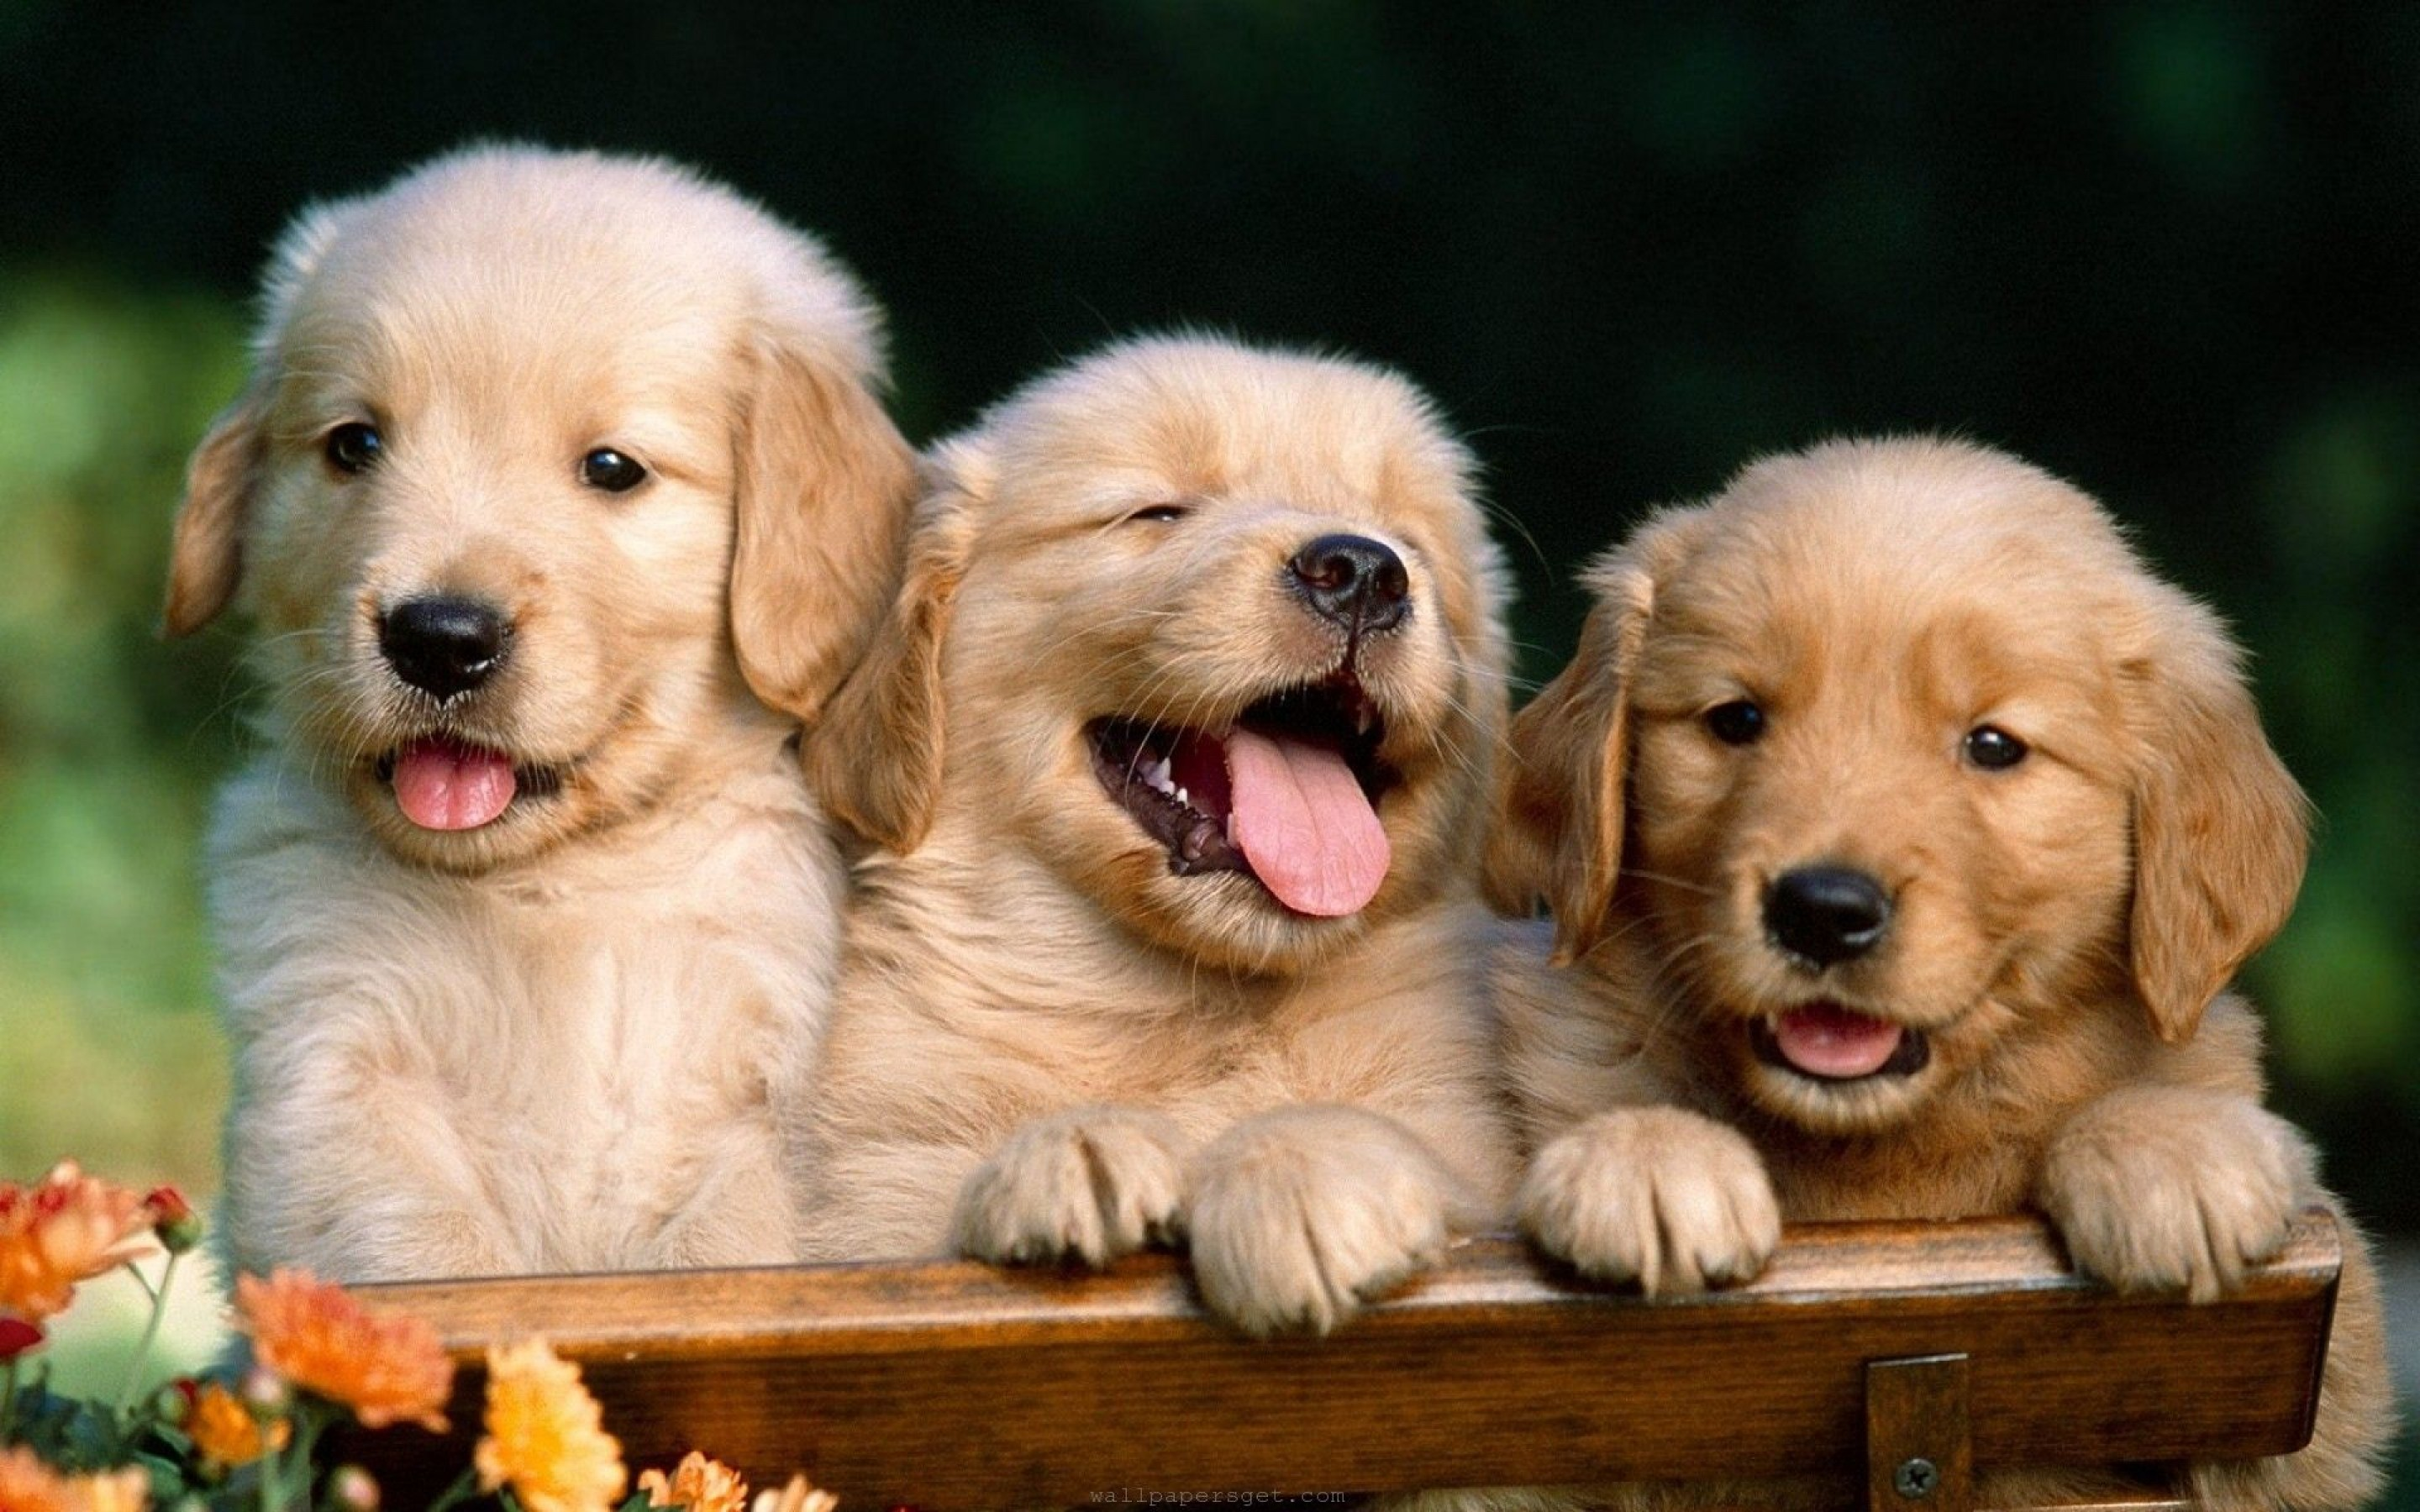
\includegraphics[width=0.8\textwidth]{Cute-Dog-Photo.jpg}
        \caption{An example cute dog image}
        \label{fig:Cute-Dog-Photo-jpg}
    \end{figure}

    \subsection{Subsection with Arrays}%
    \label{sub:Subsection with Arrays}
    
    In a table body columns are separated using an ampersand \& and a new row is started using \\.

    \begin{tabular}{lll}
    Animal & Food  & Size   \\
    dog    & meat  & medium \\
    horse  & hay   & large  \\
    frog   & flies & small  \\
    \end{tabular}

    \subsection{Table with lot of text}%
    \label{sub:Table with lot of text}
   
    If a table column contains a lot of text you will have issues to get that right with only l, c, and r. See what happens in the following example:

    \begin{tabular}{cp{9cm}}
      Animal & Description \\
      dog    & The dog is a member of the genus Canis, which forms part of the
               wolf-like canids, and is the most widely abundant terrestrial
               carnivore. \\
      cat    & The cat is a domestic species of small carnivorous mammal. It is the
               only domesticated species in the family Felidae and is often referred
               to as the domestic cat to distinguish it from the wild members of the
               family. \\
    \end{tabular}

    Adding of rules.

    \begin{tabular}{lll}
      \toprule
      Animal & Food  & Size   \\
      \midrule
      dog    & meat  & medium \\
      horse  & hay   & large  \\
      frog   & flies & small  \\
      \bottomrule
    \end{tabular}

    
    More rules.

    \begin{tabular}{lll}
      \toprule
      Animal & Food  & Size   \\
      \midrule
      dog    & meat  & medium \\
      \cmidrule{1-2}
      horse  & hay   & large  \\
      \cmidrule{1-1}
      \cmidrule{3-3}
      frog   & flies & small  \\
      \bottomrule
    \end{tabular}

    subsection{Merging of cells}

    In LaTeX you can merge cells horizontally by using the multicolumn command. It has to be used as the first thing in a cell. multicolumn takes three arguments:

    \begin{itemize}
        \item The number of cells which should be merged
        \item The alignment of the merged cell
        \item The contents of the merged cell
    \end{itemize}

    The alignment can contain anything legal in a tabular’s preamble, but only a single column type.

    \begin{tabular}{lll}
      \toprule
      Animal & Food  & Size   \\
      \midrule
      dog    & meat  & medium \\
      horse  & hay   & large  \\
      frog   & flies & small  \\
      fuath  & \multicolumn{2}{c}{unknown} \\
      \bottomrule
    \end{tabular}

    \begin{tabular}{lll}
      \toprule
      Group     & Animal & Size   \\
      \midrule
      herbivore & horse  & large  \\
                & deer   & medium \\
                & rabbit & small  \\
      \addlinespace
      carnivore & dog    & medium \\
                & cat    & small  \\
                & lion   & large  \\
      \addlinespace
      omnivore  & crow   & small  \\
                & bear   & large  \\
                & pig    & medium \\
      \bottomrule
    \end{tabular}

    \subsection{Using color boxes and borders}
    The example shows how to use the \texttt{xcolor} package 
    to change the color of \LaTeX{} page elements.

    \begin{itemize}
    \color{ForestGreen}
    \item First item
    \item Second item
    \end{itemize}
    
    \noindent
    {\color{RubineRed} \rule{\linewidth}{0.5mm}}

    The background color of text can also be \textcolor{red}{easily} set. For instance, you can change use an \colorbox{BurntOrange}{orange background} and then continue typing.

    A colored background box may be created using \verb|\colorbox{Color}{Text}| as shown here.
    For example the word "Colored Text" on a pink background \colorbox{pink}{Colored Text}.

    Another example, \colorbox{Maroon}{\textcolor{Goldenrod}{Gold color text on maroon background}}

    
    Colored and framed equations can be specified using the \verb|\fcolorbox| option as shown here:

    \[
    \fcolorbox{red}{white}{$a^{2} + b^{2} = c^{2}$}
    \]

    Colored and framed listings are possible as well:

    \fcolorbox{red}{white}{
    \parbox{0.3\textwidth}{
    \begin{itemize}
    \item listing
    \item key point 1
    \item key point 2
    \end{itemize}}
    }


    \fcolorbox{blue}{white}{
    \parbox{0.3\textwidth}{
    \begin{enumerate}
    \item enumeration
    \item key point
    \item key point
    \end{enumerate}}
    }

    \section{All Mathematics}%
    \label{sec:All Mathematics}
    
    A sentence with inline mathematics: $y = mx + c$.

    A second sentence with inline mathematics: $5^{2}=3^{2}+4^{2}$.

    A second paragraph containing display math.

    \[
        y = mx + c
    \]

    See how the paragraph continues after the display.

    Superscripts $a^{b}$ and subscripts $a_{b}$.

    Some mathematics: $y = 2 \sin \theta^{2}$.

    A paragraph about a larger equation.
    \[
        \int_{{-\infty}}^{{+\infty}} {e^{-x^2}} \, d{x}
    \]
    
    \subsection{AMSMath package}%
    \label{sub:amsmath-package}
    Mathematical notation is very rich, and this means that the tools built into the LaTeX kernel can’t cover everything. The \textit{amsmath} package extends the core support to cover a lot more ideas. The \texttt{amsmath User Guide} contains many more examples than we can show in this lesson.

    Solve the following recurrence for $ n,k\geq 0 $:
    \begin{align*}
        \label{eq:amsmath-equation}
        Q_{n,0} &= 1   \quad Q_{0,k} = [k=0];  \\
        Q_{n,k} &= Q_{n-1,k}+Q_{n-1,k-1}+\binom{n}{k} \quad\text{for $n$, $k>0$.}
    \end{align*}

    \verb|\align*| environment makes the equations line up on the ampersands, the \& symbols, just like a table. Notice how we’ve used \verb|\quad| to insert a bit of space, and \verb|\text| to put some normal text inside math mode. We’ve also used another math mode command, \verb|\binom|, for a binomial.

    Notice that here we used \verb|align*|, and the equation didn’t come out numbered. Most math environments number the equations by default, and the starred variant (with a *) disables the numbering.

    The package also has several other convenient environments, for example for matrices.

    \[
    \begin{matrix}
        a & b & c \\
        d & e & f
    \end{matrix}
    \quad
    \begin{pmatrix} 
    a & b & c \\
    a & e & f
    \end{pmatrix} 
    \quad
    \begin{bmatrix} 
    a & b & c \\
    a & e & f
    \end{bmatrix} 
    \]

    \subsection{Fonts in Math mode}%
    \label{sub:fonts-in-math}
    
    Unlike normal text, font changes in math mode often convey very specific meaning. They are therefore often written explicitly. There are a set of commands you need here:
    \begin{itemize}
        \item \verb|\mathrm|: roman (upright)
        \item \verb|\mathit|: italic spaced as ‘text’
        \item \verb|\mathbf|: bold face
        \item \verb|\mathsf|: sas serif
        \item \verb|\mathtt|: monospaced (typewriter)
        \item \verb|\mathbb|: double-struck (blackboard bold) (provided by the amsfonts package)
    \end{itemize}

    Each of these takes Latin letters as an argument, so for example we might write a matrix as

    "The matrix $\mathbf{M}$"

    \section{Paragraph spacing}%
    \label{sec:para-space}
    One common style is to have no indents for paragraphs, but instead to have a ‘blank line’ between them. We can achieve that using the \textit{parskip} package.

    \lipsum[1]

    \section{PGF Plotting}%
    \label{sec:pdf-plotting}
    We are following a sample from \url{https://latexdraw.com/plot-a-function-and-data-in-latex/}. Additional details and documentation are available at \url{https://github.com/pgf-tikz/pgfplots}.

    It is important to use the command \verb|\pgfplotsset{compat = newest}| to specify to the compiler that we are working with the last version of the Pgfplots package.

    \subsection{The plotting of equations}%
    \label{sub:plotting-figures}
    
    In order to start plot functions and data in \textrm{TikZ} we need to create the axis environment within the \textsf{tikzpicture} environment. All the \textsf{pgfplots} commands must be inside the axis environment.
    
    \begin{tikzpicture}
    \begin{axis}[]
        % here comes the picture code and an empty plot is produced
        % if we do not mention addplot here
        \addplot[] {exp(-x/10)*( cos(deg(x)) + sin(deg(x))/10 )};
    \end{axis}
    \end{tikzpicture}

    Updating the picture with proper domain and range values as the same are auto determined in the earlier case. We have the below options for changing the plot limits:

    \begin{itemize}
        \item \textit{xmin=<value>}: Lower limit in the x-axis for the plot.
        \item \textit{xmax=<value>}: Upper limit in the x-axis for the plot.
        \item \textit{ymin=<value>}: Lower limit in the y-axis for the plot.
        \item \textit{ymax=<value>}: Upper limit in the y-axis for the plot.
    \end{itemize}

    The domain of the function is independent of the limits of the axes, but usually it takes the same values to get a plot that fills the axis and it takes the format \textsf{domain = a:b}.

    \begin{tikzpicture}
    % updating the limits for axis
    \begin{axis}[
        xmin = 0,
        xmax = 30,
        ymin = -1.5,
        ymax = 2.0
        ]
        % here comes the picture code and an empty plot is produced
        % if we do not mention addplot here
        \addplot[
            domain = 0:30
        ] {exp(-x/10)*( cos(deg(x)) + sin(deg(x))/10 )};
    \end{axis}
    \end{tikzpicture}

    We can further customize the plot by setting the smoothness, thickness and color etc., as shown below:

    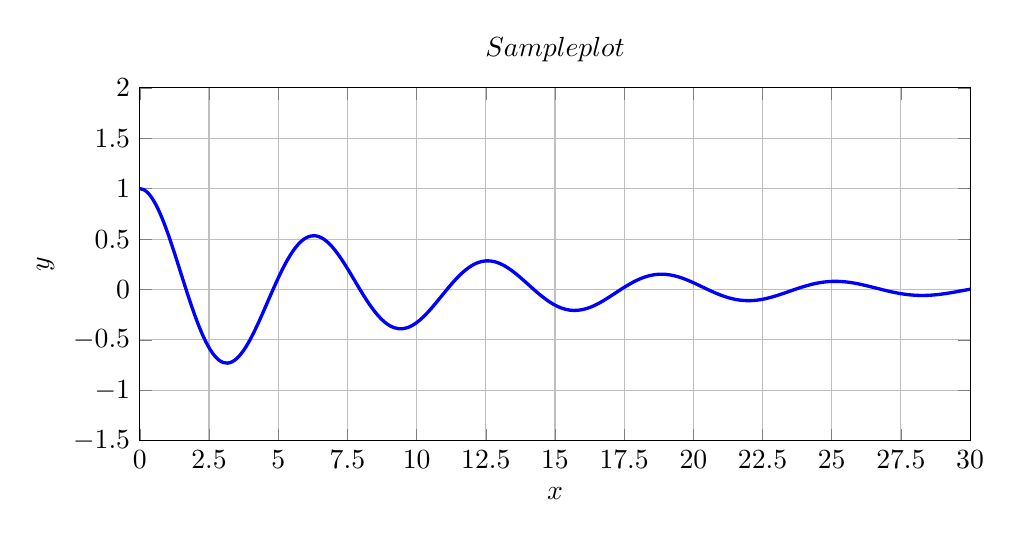
\begin{tikzpicture}
    % updating the limits for axis
    % also specifyin options to control grid and size of plot
    \begin{axis}[
        title = {$Sample plot$},
        xmin = 0, xmax = 30,
        ymin = -1.5, ymax = 2.0,
        xtick distance = 2.5,
        ytick distance = 0.5,
        grid = both,
        major grid style = {lightgray},
        minor grid style = {lightgray!25},
        width = \textwidth,
        height = 0.5\textwidth,
        xlabel = $x$,
        ylabel = $y$,
        ]
        % here comes the picture code and an empty plot is produced
        % if we do not mention addplot here
        \addplot[
            domain = 0:30,
            samples = 200,
            smooth,
            very thick,
            blue,
        ] {exp(-x/10)*( cos(deg(x)) + sin(deg(x))/10 )};
    \end{axis}
    \end{tikzpicture}

    % Preamble: \pgfplotsset{width=7cm,compat=1.18}
    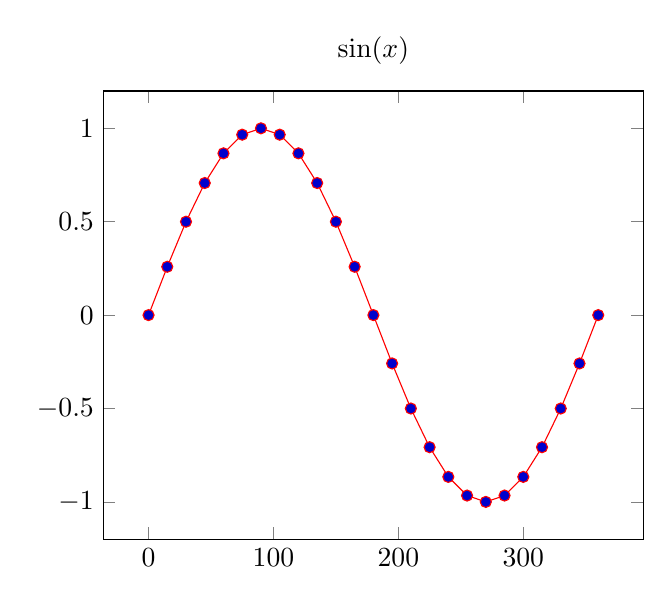
\begin{tikzpicture}
        \begin{axis}[
            title={$\sin(x)$}
            ]
        \addplot+ [
            domain=0:360,
            red,
        ] {sin(x)};
    \end{axis}
    \end{tikzpicture}

    \subsection{Adding captions and labelling}%
    \label{sub:captions-labelling}
    
    We can provide names or labels to the generated figures as demonstrated here

    \begin{figure}[hbt!]
        \centering
        \resizebox{0.6\textwidth}{!}{%
            
\begin{tikzpicture}
                \draw[fill=yellow!50] (0,0) circle [radius=2];
                \draw[fill=pink] (-0.5,0.5,0) ellipse [x radius=0.2, y radius=0.4];
                \draw[fill=pink] (0.5,0.5,0) ellipse [x radius=0.2, y radius=0.4];
                \draw[very thick] (-1,-1) arc [start angle=185, end angle=355, x radius=1, y radius=0.5];
            \end{tikzpicture}
        }
        \caption{Set of balls}
        \label{fig:balls}
    \end{figure}


\newpage
\bibliographystyle{plainnat}
\bibliography{learnlatex}
\end{document}
